\documentclass[12pt]{cpthesis}

%% Math packages
\usepackage{amssymb}
\usepackage{amsmath}

%% Figures and tables packages
\usepackage{tabularx}
\usepackage{graphicx}
% Add figures folder to the graphics path
\graphicspath{{figures/}}
% Ensures table floats have caption above table.
% from https://tex.stackexchange.com/a/43097
% Note: Still have to manually do this for non-floating tables.
\usepackage{floatrow}
\floatsetup[table]{capposition=top}

%% Bibliography packages
\bibliographystyle{abbrv}

%% hyperlinks and URL handling
%% Note: must be one of the last packages added
\usepackage[hyphens]{url}
\usepackage[breaklinks=true,hidelinks,pdfusetitle]{hyperref}
% Options for hyperref
\hypersetup{
    bookmarksnumbered=true,
    bookmarksopen=false,
    bookmarksopenlevel=0,
    colorlinks=false,
    pdfstartview=Fit,
    pdfborder={0 0 0},
}
% remove \uppercase from references to chapters
% see: https://tex.stackexchange.com/a/417078
\pdfstringdefDisableCommands{\let\uppercase\@firstofone}

%% Automatic determination of kind of reference
%% Note: must be included after hyperref
\RequirePackage{cleveref}
% Define Appendix refs
\crefname{app}{appendix}{appendices}
\Crefname{app}{Appendix}{Appendices}

%% Only needed to create placeholder text
\usepackage{lipsum}

%% Setting for the front matter
\title{Your Thesis Title}
\author{Your Name}
\degreemonth{June} \degreeyear{2014} \degree{Master of Science}
\defensemonth{June} \defenseyear{2014}
\numberofmembers{2}
   \chair{Alexander Dekhtyar, Ph.D. \linebreak Professor of Computer Science}
   \othermemberA{Aaron Keen, Ph.D. \linebreak Professor of Computer Science}
   \othermemberB{Franz Kurfess 3, Ph.D. \linebreak Professor of Computer Science}
   \othermemberC{Franz Kurfess 4, Ph.D. \linebreak Professor of Computer Science}
   \othermemberD{Franz Kurfess 5, Ph.D. \linebreak Professor of Computer Science}
   \othermemberE{Franz Kurfess 6, Ph.D. \linebreak Professor of Computer Science}
   \othermemberF{Franz Kurfess 7, Ph.D. \linebreak Professor of Computer Science}
   \othermemberG{Franz Kurfess 8, Ph.D. \linebreak Professor of Computer Science}
   \othermemberH{Franz Kurfess 9, Ph.D. \linebreak Professor of Computer Science}
   \othermemberI{Franz Kurfess 10, Ph.D. \linebreak Professor of Computer Science}
\field{Computer Science} \campus{San Luis Obispo}
\copyrightyears{seven}
\keywords{Select descriptive keywords and separate terms with a comma and a space.}



\begin{document}
    \begin{frontmatter}
        \maketitle

        % Custom made for Cal Poly (by Mark Barry, modified by Andrew Tsui).
        \copyrightpage

        % Custom made for Cal Poly (by Andrew Tsui).
        \committeemembershippage

        % Abstract page
        \begin{abstract}
            Your abstract goes in here.
\lipsum[1-2]

        \end{abstract}

        % Acknowledgments page
        % Note: environment is included in the tex-file so can change
        % page title if needed.
        % if only have one acknowledgment then uncomment this line
%\renewcommand{\acknowledgename}{Acknowledgment}

\begin{acknowledgments}

    This page is optional, but if you have received funding for your research or assistance or guidance that you feel should be noted, it belongs on this page. If you are not including acknowledgments, delete this page. If you are acknowledging only one person, change the title to ACKNOWLEDGMENT by removing commented line in acknowledgments file.

    Thanks to:
    \begin{itemize}
        \item Andrew Guenther, for uploading this template, and
        \item Someone Else, so that I do not have to rename this page.
    \end{itemize}
\end{acknowledgments}


        \begin{dedication}
            This is optional, but can be included if desired.
        \end{dedication}

        \tableofcontents

        \listoftables

        \listoffigures
    \end{frontmatter}

    %% Input the chapters as configured from the file
    \chapter{Example Usage} \label{sec:ExampleUsage}
    This chapter is an introduction to the various elements of a thesis that might need to be created.
    Any additional packages beyond what is already included in the main \LaTeX\ file should be put into the preamble.tex file located in the frontmatter directory.

\section{Math} \label{sec:Math}
    Displaying math relations is one of the areas that \LaTeX\ shines.
    While this is not a complete presentation of the capabilities, there are a few uses that are worth presenting as a starting point.

\subsection{General Equations}
    This section shows how to create a variety of equations and cite them.
    \Cref{eq:quadratic_formula} is an example of a simple equation.
    \begin{equation} \label{eq:quadratic_formula}
        x=\frac{-b\pm\sqrt{b^2-4ac}}{2a}
    \end{equation}
    For equations that are not to be numbered, then can use the ``*'' version of the math commands, such as
    \begin{equation*}
        y=mx+b
    \end{equation*}
    Note that since this equation is not numbered, it cannot be referenced in the text because it has no label.

    For one equation that splits over multiple lines, \cref{eq:multi_line} can be used as a reference
    \begin{equation} \label{eq:multi_line}
        \begin{split}
            x&=\frac{-b\pm\sqrt{b^2-4ac}}{2a}
              =\frac{-b\pm\sqrt{b^2-4ac}}{2a}\left(\frac{-b\mp\sqrt{b^2-4ac}}{-b\mp\sqrt{b^2-4ac}}\right) \\
             &=\frac{b^2-\left(b^2-4ac\right)}{2a\left(-b\mp\sqrt{b^2-4ac}\right)}
              =\frac{4ac}{2a\left(-b\mp\sqrt{b^2-4ac}\right)} \\
             &=-\frac{2c}{b \pm \sqrt{b^2-4ac}}
        \end{split}
    \end{equation}

    If you have multiple equations that are related then can use the following
    \begin{subequations} \label{eq:subeq_example}
        \begin{align}
            \begin{split}
                q\left(x\right)&\coloneq\frac{6x^2}{2x} \\
                &=3x
            \end{split} \label{eq:subeq1} \\
            q\left(1\right)
                &=3\cdot 1=3 \label{eq:subeq2} \\
            q\left(0\right)
                &=\lim_{x\to 0} q=0 \label{eq:subeq3}
        \end{align}
    \end{subequations}
    where each sub-equation can referred to individually, such as \cref{eq:subeq2}, as a collection, such as \cref{eq:subeq1,eq:subeq2,eq:subeq3}, or as the entire set of equations, such as \cref{eq:subeq_example}.
    In the case that some of the equations should not be numbered, then can use the \textbackslash notag command on the equations that should not be numbered
    \begin{subequations}
        \begin{align}
            \begin{split}
                q\left(x\right)
                    &\coloneq\frac{6x^2}{2x} \\
                    &=3x
            \end{split} \\
            q\left(1\right)
                &=3\cdot 1=3 \notag \\
            q\left(0\right)
                &=\lim_{x\to 0} q=0
        \end{align}
    \end{subequations}

\subsection{Functions and Their Names}
    It is important to remember that math functions, such as sine and cosine, have their own definitions, and are typeset differently compared to variables.
    \begin{equation}
        \sin\left(2\alpha\right)=2\sin\left(\alpha\right)\cos\left(\alpha\right)
    \end{equation}
    Any math function that is represented by multiple characters should follow the same formatting.
    To create custom math functions, use the \textbackslash DeclareMathOperator command.

\subsection{Representing Vectors}
    Vectors are represented a variety of ways in different fields of study.
    A few of the most common methods are presented here.

\subsubsection{Vectors as Bold Symbols}
    A three-dimensional vector has the form
    \begin{equation}
        \bm{x}
            =\begin{bmatrix}
                x_0 \\ x_1 \\ x_2
             \end{bmatrix}
    \end{equation}
    while a row vector looks like
    \begin{equation}
        \bm{\alpha}
            =\begin{bmatrix}
                \alpha_0 & \alpha_1 & \alpha_2
             \end{bmatrix}
    \end{equation}
    The same process can be used to represent a matrix
    \begin{equation}
        \bm{\mu}
            =\begin{bmatrix}
                \bm{\mu}_0 & \bm{\mu}_1 & \bm{\mu}_{2}
             \end{bmatrix}
            =\begin{bmatrix}
                \mu_{0,0} & \mu_{0,1} & \mu_{0,2} \\
                \mu_{1,0} & \mu_{1,1} & \mu_{1,2} \\
                \mu_{2,0} & \mu_{2,1} & \mu_{2,2} \\
             \end{bmatrix}
    \end{equation}

\subsubsection{Vectors with Arrows Above}
    A three-dimensional vector has the form
    \begin{equation}
        \vec{x}
            =\begin{bmatrix}
                x_0 \\ x_1 \\ x_2
             \end{bmatrix}
    \end{equation}
    while a row vector looks like
    \begin{equation}
        \vec{\alpha}
            =\begin{bmatrix}
                \alpha_0 & \alpha_1 & \alpha_2
             \end{bmatrix}
    \end{equation}
    The same process can be used to represent a matrix
    \begin{equation}
        \vec{\mu}_i
            =\begin{bmatrix}
                \vec{\mu}_0 & \vec{\mu}_1 & \vec{\mu}_{2}
             \end{bmatrix}
            =\begin{bmatrix}
                \mu_{0,0} & \mu_{0,1} & \mu_{0,2} \\
                \mu_{1,0} & \mu_{1,1} & \mu_{1,2} \\
                \mu_{2,0} & \mu_{2,1} & \mu_{2,2} \\
             \end{bmatrix}
    \end{equation}

\subsubsection{Vectors with Lines Below}
    A three-dimensional vector has the form
    \begin{equation}
        \underline{x}
            =\begin{bmatrix}
                x_0 \\ x_1 \\ x_2
             \end{bmatrix}
    \end{equation}
    while a row vector looks like
    \begin{equation}
        \underline{\alpha}
            =\begin{bmatrix}
                \alpha_0 & \alpha_1 & \alpha_2
             \end{bmatrix}
    \end{equation}
    The same process can be used to represent a matrix
    \begin{equation}
        \underline{\underline{\mu}}
            =\begin{bmatrix}
                \underline{\mu_0} & \underline{\mu_1} & \underline{\mu_2}
             \end{bmatrix}
            =\begin{bmatrix}
                \mu_{0,0} & \mu_{0,1} & \mu_{0,2} \\
                \mu_{1,0} & \mu_{1,1} & \mu_{1,2} \\
                \mu_{2,0} & \mu_{2,1} & \mu_{2,2} \\
             \end{bmatrix}
    \end{equation}

\section{Figures} \label{sec:Figures}
    Figures are typically included as either images or drawings.
    There are a number of image and drawing formats that can be used, however this will only present a few figure format types.
    If your thesis has no figures, then the list of figures should be removed from the thesis.
    This is accomplished by removing the code in listings.tex associated with the list of figures.

\subsection{Figures from Images} \label{sec:FiguresFromImages}
    Image files can be inserted using the \textbackslash includegraphics command.
    \Cref{fig:CalPolySeal1} shows the import of a JPG file at its original size.
    The default size of this image is quite large, and the scale does not add much value.
    There are a number of ways to scale an image, with \cref{fig:CalPolySeal_small} showing one way to do so.
    This figure scaled the image to a width of 2 inches.
    \makeatletter
    \@currsize
    \makeatother
    \begin{figure}
        \centering
        
\includegraphics{CalPoly_Seal}
        \caption{The Cal Poly seal.}
        \label{fig:CalPolySeal1}
    \end{figure}
    \begin{figure}
        \centering
        
\includegraphics[width=2in]{CalPoly_Seal}
        \caption{The Cal Poly seal from \cref{fig:CalPolySeal1} scaled to a 2 inch width.}
        \label{fig:CalPolySeal_small}
    \end{figure}

    Beware that scaling images can result in the image looking quite poor.
    \Cref{fig:CalPolySeal_scaled} shows a small version of the Cal poly seal that was then scaled to a width of 2 inches.
    Note how pixelated the resulting image is, and it is difficult to determine what the actual image should be.\footnote{Too many technical documents suffer from the problem of pixelated images in their figures, including textbooks, unfortunately.}
    It is best practice to save the image at the resolution that you plan to use in your document.
    This takes some iterations to get the sizes correct, but it will create much better looking images.
    \begin{figure}
        \centering
        
\includegraphics[width=2in]{CalPoly_Seal_small}
        \caption{A small version of the Cal Poly seal scaled to a 2 inch width as an example of a poorly formatted image for a figure.}
        \label{fig:CalPolySeal_scaled}
    \end{figure}

\subsection{Figures from TikZ} \label{sec:FiguresFromTikZ}
    Another way to present figures is to use one of the drawing packages compatible with \LaTeX.
    One such solution is TikZ.\footnote{TikZ is a drawing package that has many extensions and uses. A good website to start with is \url{https://tikz.dev/}.}
    \Cref{fig:tikz_drawing} shows a simple drawing made using TikZ.
    The code for drawing can either be placed in the \TeX--file, or it can be included from another file, as this example.
    One benefit of using TikZ (and other \LaTeX--based drawing packages) is that the same fonts are used in the drawing as are used in the rest of the document.
    So there are no issues with the distraction of each figure having its own fonts (and sizes).
    \begin{figure}
        \centering
        \begin{tikzpicture}[scale=1.25]
    \def\c {4cm}
    \def\t {2cm}
    \def\shockheight {3cm}
    \coordinate (leading edge) at (0, 0);
    \coordinate (upper end) at (\c, \t);
    \coordinate (lower end) at (\c, -\t);

    % draw the surfaces
    \draw[opacity=0.5, fill=gray, gray] (leading edge) -- (upper end) to[out=-10,in=145] (lower end) -- cycle;
    \draw[thick] (lower end) -- (leading edge) -- (upper end);
    \node[xshift=-2cm] at ($(upper end)!0.5!(lower end)$) {Generic Cone};

    % draw shocks
    \draw[very thick] (leading edge) -- ++(-50:\shockheight) node[sloped, midway, below] {$y=mx+b$};
    \draw[very thick] (leading edge) -- ++(50:\shockheight);
\end{tikzpicture}

        \caption{A simple TikZ drawing demonstrating its use.}
        \label{fig:tikz_drawing}
    \end{figure}

    Another example of TikZ usage is \cref{fig:tikz_venn} from \cite{kottwitz2015}.
    This demonstrates the versatility of TIkZ to produce a wide variety of figures.
    There are a number of other ways that TikZ can be used to create figures for plots (using pgfplots), circuits (using circuitikz), and structural analysis (using stanli).
    \begin{figure}
        \centering
        % A Venn diagram with PDF blending
% Author: Stefan Kottwitz
% https://www.packtpub.com/hardware-and-creative/latex-cookbook
%
% Retrieved from https://texample.net/tikz/examples/venn/
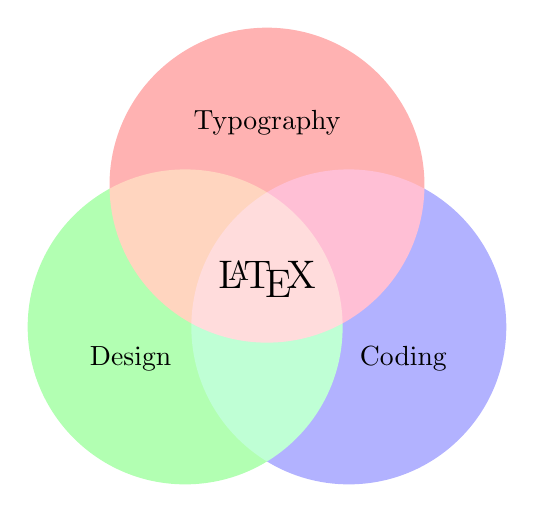
\begin{tikzpicture}
    \begin{scope}[blend group = soft light]
        \fill[red!30!white]   ( 90:1.2) circle (2);
        \fill[green!30!white] (210:1.2) circle (2);
        \fill[blue!30!white]  (330:1.2) circle (2);
    \end{scope}
    \node at ( 90:2)    {Typography};
    \node at ( 210:2)   {Design};
    \node at ( 330:2)   {Coding};
    \node [font=\Large] {\LaTeX};
\end{tikzpicture}

        \caption{A Venn diagram describing \LaTeX created by Stefan Kottwitz\cite{kottwitz2015}.}
        \label{fig:tikz_venn}
    \end{figure}

\subsection{Sub-Figures}
    Sometimes there is a need to present the contents of two images/drawing together in one figure.
    \Cref{fig:subfig-example} shows a figure composed of two sub-figures.
    Each sub-figure can be referred to separately, such as \cref{fig:sub-image-a} is on the left and \cref{fig:sub-image-b} is on the right.
    Also, the sub-figures can be cited collectively, such as \cref{fig:sub-image-a,fig:sub-image-b}.
    \begin{figure}
        \centering
        \begin{subfigure}[t]{2.5in}
            \includegraphics[width=\textwidth]{example-image-a}
            \caption{First example image that does have a long description.}
            \label{fig:sub-image-a}
        \end{subfigure}
        \hspace{0.2in}
        \begin{subfigure}[t]{2.5in}
            \includegraphics[width=\textwidth]{example-image-b}
            \caption[size=normal]{Another example image with a long description that continues on for a while.}
            \label{fig:sub-image-b}
        \end{subfigure}
        \caption{Two figures that together tell a complete story of how sub-figures can be used together to create one coherent figure.}
        \label{fig:subfig-example}
    \end{figure}

\section{Tables} \label{sec:Tables}
    Tables are handled similarly to figures within \LaTeX.
    If your thesis has no tables, then the list of tables should be removed from the thesis.
    This is accomplished by removing the code in listings.tex associated with the list of tables.

    One exception is that the caption for a table should be above the table, while the caption for figures should be below the figure.
    Table~\ref{tab:fancy-table-example} shows a floating table with a variety of column types.
    The formatting for these columns (such as aligning floating point numbers on the decimal, scientific notation, and unit labels) can be accomplished using the siunitx package, however that is beyond the scope of this introduction.
    \begin{table}
        \centering
        \begin{tabular}{c l l l l}
                      & \multicolumn{1}{c}{Ref.}& \multicolumn{1}{c}{Calc.}& \multicolumn{1}{c}{Absolute}& \multicolumn{1}{c}{Percent} \\
            Parameter & \multicolumn{1}{c}{Value}& \multicolumn{1}{c}{Value}& \multicolumn{1}{c}{Difference}& \multicolumn{1}{c}{Difference (\%)} \\
            \hline
            Radius & 150.0 & 150.0 & $\phantom{-}0.000\times 10^{0}$ & \quad\quad 0.0 \\
            Chord & \phantom{1}60.00 & \phantom{1}60.00 & $\phantom{-}0.000\times 10^{0}$ & \quad\quad 0.0 \\
            Thickness & \phantom{15}6.000 & \phantom{15}6.061 & $\phantom{-}6.123\times 10^{-2}$ & \quad\quad 1.021 \\
            $\theta_\text{l.e.}\ \left(^\circ\right)$ & \phantom{1}11.33 & \phantom{1}11.54 & $\phantom{-}2.036\times 10^{-1}$ & \quad\quad 1.797 \\
            $\theta_\text{t.e.}\ \left(^\circ\right)$ & \,-11.33 & \,-11.54 & $-2.036\times 10^{-1}$ & \quad\quad 1.797 \\
            \hline
        \end{tabular}
        \caption{The formatting of this table is hackish. There are better ways to align numbers. The siunitx package provides this feature.}
        \label{tab:fancy-table-example}
    \end{table}

    While there are a number of formatting options for tables, be careful that the resulting formatting still adheres to the thesis formatting guidelines.
    In addition, a general rule for horizontal and vertical lines is the fewer the better.
    In particular, vertical lines should be used on the rarest of occasions.
    Horizontal lines should be used sparingly as well, but should be used to delineate the column headings.
    Adding horizontal lines at the top and bottom of the table are up to your discretion.
    Whatever formatting you adopt, be sure to be consistent throughout the entire thesis.

\subsection{Sub-Tables}
    Just as the case with figures in \cref{sec:Figures}, there are some occasions that might necessitate the need for two tables to be presented in one table.
    Note that this is a rarer need than with sub-figures, so be judicious with the usage of sub-tables.
    \Cref{tab:temps} is a table composed of two sub-tables.
    Each sub-table can be referred to separately, such as \cref{tab:week1} is for the first week and \cref{tab:week2} is for the second week.
    These sub-tables can be cited collectively as well, such as \cref{tab:week1,tab:week2}.
    \begin{table}
        \begin{subtable}[h]{0.375\textwidth}
            \centering
            \caption{First week temperatures.}
            \label{tab:week1}
            \begin{tabular}{r r r}
                      & Min.  & Max. \\
                Day   & $\left(^\circ\text{C}\right)$
                              & $\left(^\circ\text{C}\right)$ \\
                \hline
                Mon   & 13 & 20 \\
                Tue   & 14 & 22 \\
                Wed   & 12 & 23 \\
                Thurs & 13 & 25 \\
                Fri   & 7  & 18 \\
                Sat   & 13 & 15 \\
                Sun   & 13 & 20 \\
                \hline
            \end{tabular}
        \end{subtable}
        \hspace{0.2in}
        \begin{subtable}[h]{0.375\textwidth}
            \caption{Second week temperatures.}
            \label{tab:week2}
            \centering
            \begin{tabular}{r r r}
                      & Min.  & Max. \\
                Day   & $\left(^\circ\text{C}\right)$
                              & $\left(^\circ\text{C}\right)$ \\
                \hline
                Mon   & 11 & 17 \\
                Tue   & 10 & 16 \\
                Wed   & 8  & 14 \\
                Thurs & 5  & 12 \\
                Fri   & 7  & 15 \\
                Sat   & 12 & 16 \\
                Sun   & 9  & 15 \\
                \hline
            \end{tabular}
        \end{subtable}
        \caption{Temperature ranges recorded in the first two weeks of July at the first station in study.}
        \label{tab:temps}
    \end{table}

\section{Cross-References} \label{sec:CrossReferences}
    There are many ways that cross-references can be created in the document.
    The package that this document uses is cleveref.
    The \textbackslash cref, cross-reference in a sentence, and \textbackslash Cref, cross-reference to start a sentence, commands have already been used throughout this chapter.
    As an example, \cref{sec:ExampleUsage} has a section titled \nameref{sec:FiguresFromImages}, located inside \cref{sec:Figures} on \cpageref{sec:FiguresFromImages}.
    The chapter and number, the section title, the section and number, and the page number were all created using cleveref cross-references.
    If in the future the chapter number, section title, section number, and/or page number change these will be updated automatically.
    There should be no reason to ever manually cross-reference an item in this document.

\section{Nomenclature Usage} \label{sec:NomenclatureUsage}
    The \nameref{sec:Nomenclature} in the preamble on \cpageref{sec:Nomenclature} shows the nomenclature for this document.
    This uses the nomencl package, and you should consult the documentation for that package to see how it can be customized.
    The simplest way to implement the nomenclature/list of symbols information is how this document has created the nomenclature.
    All of the nomenclature information is contained within the nomenclature.tex file in the frontmatter directory.
    If no nomenclature is desired, then simply remove all of the content in this file and remove the list of symbols code in the listings.tex file.

    There are ways to sort/organize the nomenclature.
    A simple grouping is done with the code in the preamble.tex file.
    If a different sorting/grouping is desired, then this code needs to be changed.
    If no grouping or sorting is desired, then this code can be removed.

\section{Citations} \label{sec:Citations}
    This document uses biblatex and the biber bibliography parser to generate the bibliography/references section.
    The bibliography data is located in the bib-file, references.bib, located in the bibliography directory.
    This file provides a small selection of sample source types.
    There are a large number of source types that can be found in the documentation for biblatex.
    \emph{Note that since not every item in the bib-file was cited, this document has a Bibliography after the last chapter (instead of a References section if all items had been cited).}

    There are also a number of other resources that can help create source entries.
    Many publishers offer the ability to export a citation in bibtex format, and this can easily be included into the references.bib file (sometimes without any modifications).
    There are also more sophistical reference management systems, such as Zotero\footnote{ \url{https://www.zotero.org}} and Mandeley\footnote{\url{https://www.mendeley.com}}, that can export citations.
    No matter where the citation source was generated, it will probably take some fine tuning of the bib-file contents to make the cited work correctly formatted.

    The other file in the bibliography directory is the bib\_info.tex file.
    This file needs to be edited depending on whether your thesis will have a bibliography or reference section.
    A reference section contains just the items that the thesis cites.
    A bibliography includes both the cited items as well as any other valuable resources related to topics within your thesis.

    To cite an entry can be done using the \textbackslash cite command, such as \cite{cpthesis_github}.
    Multiple entries can be cited as well \cite{drela1986a,dryden1943a,einstein1905,lopez2007a}.
    Sometimes it is necessary to append some text to the citation as in \cite[135]{dryden1943a} and \cite[section 2]{head1958a}.
    You can also prepend text \cite[such as][120]{Koutsovasilis2008}.
    To refer to the author(s) and cite the \textbackslash textcite command can be used as in \textcite{dirac1981}.
    Finally, other parts of the citation can also be referenced: \citeauthor{einstein1905} wrote \citetitle{einstein1905} in \citeyear{einstein1905} with the citation found in \cite{einstein1905}.

\section{Algorithms} \label{sec:Algorithms}
    When there is a need to demonstrate an algorithm the algorithmic package can be used.
    \Cref{alg:SecondAlgorithm} shows a simple example of an algorithm.
    This one does not contain comments and is a more stripped-down example of the features of the algorithmic package.
    \begin{algorithm}
        \begin{algorithmic}
            \Require $x \in \{0,1\}$
            \Ensure $y \in \{1,2\}$
            \State $y \gets x+1$
            \State \Return $y$
        \end{algorithmic}
        \caption{Another algorithm.}
        \label{alg:SecondAlgorithm}
    \end{algorithm}

    Another algorithm is shown as a simple implementation of Heun's Method in \cref{alg:HeunMethod}.
    This computes solutions to $y'=f\left(x,y\right)$ at $N$ locations with step-size $h$, and initial value of $x_0, y_0$.
    References can be made to specific lines in the algorithm.
    In this case, \cref{alg:HeunMethodPredictor} shows the predictor step.
    \begin{algorithm}
        \begin{algorithmic}
            \Require $f\left(x,y\right)$, $N\in\mathbb{N}$
            \Procedure{HeunMethod}{$f, x_0, y_0, h, N$}
                \For{$n\gets 0, N-1$}\Comment{looping through $N$ evaluations}
                    \State $x_{n+1}\gets x_n+h$\Comment{Setting the next $x$}
                    \State $K_1\gets hf\left(x_n, y_n\right)$\Comment{Store the evaluation of $f$}
                    \State $y^*\gets y_n+K_1$\Comment{Predictor Calculation} \label{alg:HeunMethodPredictor}
                    \State $K_2\gets hf\left(x_{n+1}, y^*\right)$\Comment{Store second evaluation of $f$}
                    \State $y_{n+1}\gets y_n+\frac{1}{2}\left[K_1+K_2\right]$\Comment {Corrector Calculation}
                \EndFor
                \State \textbf{return} $x,y$ \Comment{return the $x$ and $y$ vectors}
            \EndProcedure
        \end{algorithmic}
        \caption{Heun's Method for given step-size.}
        \label{alg:HeunMethod}
    \end{algorithm}

\section{Code and Code Listings} \label{sec:CodeAndCodeListings}
    When code needs to be included in the document, it is important to use a mono-spaced font because many programming languages use spaces to indicate subordinate code.
    The listing package automatically selects the appropriate font so that the mono-spaced font is not jarringly different from the rest of the text font, similarly to how the math font is chosen to work well with the text font.
    Ideally, it would be nice to differentiate inline code so that it is clear that \textbackslash incmatrix is a function defined in code, however the thesis format requires the same font for all text.
    \Cref{lst:OverleafCode}, shows an example python code originally from Overleaf.\footnote{Complete example can be found at \url{https://www.overleaf.com/learn/latex/Code_listing}}
    This code is in a floating environment (note the usage of the float option).\footnote{To enforce the placement of the listing in this example, the ``h'' parameter is used. In general no placement parameters are needed, and the ``float'' option is all that is needed to be used.}
    Without that option the code listing will appear exactly in the text where the code listing is.

    \begin{lstlisting}[float=hb, caption=Example from Overleaf demonstrating python code using a monospaced font. The use of this font is important to see what statement the return lines up with., label=lst:OverleafCode]
import numpy as np

def incmatrix(genl1,genl2):
    m = len(genl1)
    n = len(genl2)
    M = None #to become the incidence matrix
    VT = np.zeros((n*m,1), int)  #dummy variable

    #compute the bitwise xor matrix
    M1 = bitxormatrix(genl1)
    M2 = np.triu(bitxormatrix(genl2),1)

    for i in range(m-1):
        for j in range(i+1, m):
            [r,c] = np.where(M2 == M1[i,j])
            for k in range(len(r)):
                VT[(i)*n + r[k]] = 1;
                VT[(i)*n + c[k]] = 1;
                VT[(j)*n + r[k]] = 1;
                VT[(j)*n + c[k]] = 1;

                if M is None:
                    M = np.copy(VT)
                else:
                    M = np.concatenate((M, VT), 1)

                VT = np.zeros((n*m,1), int)

    return M
    \end{lstlisting}


\chapter{Generic Content}
    \lipsum[1]
    \begin{table}
        \centering
        \begin{tabular}{r r r r r r r r}
             Col1 & Col2 & Col3 & Col4 & Col1 & Col2 & Col3 & Col4 \\
             \hline
             1    & 676  & 8837 & 787  & 544  & 22   & 908  & 229  \\
             2    & 732  & 78   & 5415 & 887  & 343  & 1112 & 870  \\
             3    & 545  & 778  & 7507 & 5554 & 5432 & 9867 & 9    \\
             4    & 545  & 1874 & 7560 & 102  & 562  & 223  & 792  \\
             5    & 88   & 788  & 6344 & 45   & 998  & 776  & 2    \\
             \hline
        \end{tabular}
        \caption{This is the caption for the first table.}
    \end{table}
    \lipsum[2]

\section{A Section}
    \lipsum[3]
    \begin{table}
        \centering
        \begin{tabular}{r r r r r r r r}
             Col1 & Col2 & Col3 & Col4 & Col1 & Col2 & Col3 & Col4 \\
             \hline
             1    & 676  & 8837 & 787  & 544  & 22   & 908  & 229  \\
             2    & 732  & 78   & 5415 & 887  & 343  & 1112 & 870  \\
             3    & 545  & 778  & 7507 & 5554 & 5432 & 9867 & 9    \\
             4    & 545  & 1874 & 7560 & 102  & 562  & 223  & 792  \\
             5    & 88   & 788  & 6344 & 45   & 998  & 776  & 2    \\
             \hline
        \end{tabular}
        \caption{This is the caption for another table.}
    \end{table}
    \lipsum[4-5]
    \begin{figure}
        \centering
        \includegraphics[width=3.5in]{example-image}
        \caption{This is the caption for first image.}
    \end{figure}

\subsection{A Subsection}
    \lipsum[6-8]
    \begin{figure}
        \centering
        \includegraphics{example-image-golden}
        \caption{This is the caption for another image where the description is rather long and will probably go beyond one line.}
    \end{figure}

\section{Another Section}
    \lipsum[1-2]
    \begin{table}
        \centering
        \begin{tabular}{r r r r r r r r}
             Col1 & Col2 & Col3 & Col4 & Col1 & Col2 & Col3 & Col4 \\
             \hline
             1    & 676  & 8837 & 787  & 544  & 22   & 908  & 229  \\
             2    & 732  & 78   & 5415 & 887  & 343  & 1112 & 870  \\
             3    & 545  & 778  & 7507 & 5554 & 5432 & 9867 & 9    \\
             4    & 545  & 1874 & 7560 & 102  & 562  & 223  & 792  \\
             5    & 88   & 788  & 6344 & 45   & 998  & 776  & 2    \\
             \hline
        \end{tabular}
        \caption{This is the caption for yet another table.}
    \end{table}

\subsection{Another Subsection}
    \lipsum[3-5]

\subsubsection{A Sub-Subsection}
    \lipsum[6-8]


\chapter{Second Chapter}
    \lipsum[1]
    \begin{table}
        \centering
        \begin{tabular}{r r r r r r r r}
             Col1 & Col2 & Col3 & Col4 & Col1 & Col2 & Col3 & Col4 \\
             \hline
             1    & 676  & 8837 & 787  & 544  & 22   & 908  & 229  \\
             2    & 732  & 78   & 5415 & 887  & 343  & 1112 & 870  \\
             3    & 545  & 778  & 7507 & 5554 & 5432 & 9867 & 9    \\
             4    & 545  & 1874 & 7560 & 102  & 562  & 223  & 792  \\
             5    & 88   & 788  & 6344 & 45   & 998  & 776  & 2    \\
             \hline
        \end{tabular}
        \caption{This is the caption for a table that has a long description that does not add much to the understanding and should be shortened.}
    \end{table}
    \lipsum[2]

\section{A Section}
    \lipsum[3]
    \begin{table}
        \centering
        \begin{tabular}{r r r r r r r r}
             Col1 & Col2 & Col3 & Col4 & Col1 & Col2 & Col3 & Col4 \\
             \hline
             1    & 676  & 8837 & 787  & 544  & 22   & 908  & 229  \\
             2    & 732  & 78   & 5415 & 887  & 343  & 1112 & 870  \\
             3    & 545  & 778  & 7507 & 5554 & 5432 & 9867 & 9    \\
             4    & 545  & 1874 & 7560 & 102  & 562  & 223  & 792  \\
             5    & 88   & 788  & 6344 & 45   & 998  & 776  & 2    \\
             \hline
        \end{tabular}
        \caption{This is the caption for a table.}
    \end{table}
    \lipsum[4-5]
    \begin{figure}
        \centering
        \includegraphics[width=4in]{example-image}
        \caption{This is the caption for an image.}
    \end{figure}

\subsection{A Subsection}
    \lipsum[6-8]
    \begin{table}
        \centering
        \begin{tabular}{r r r r r r r r}
             Col1 & Col2 & Col3 & Col4 & Col1 & Col2 & Col3 & Col4 \\
             \hline
             1    & 676  & 8837 & 787  & 544  & 22   & 908  & 229  \\
             2    & 732  & 78   & 5415 & 887  & 343  & 1112 & 870  \\
             3    & 545  & 778  & 7507 & 5554 & 5432 & 9867 & 9    \\
             4    & 545  & 1874 & 7560 & 102  & 562  & 223  & 792  \\
             5    & 88   & 788  & 6344 & 45   & 998  & 776  & 2    \\
             \hline
        \end{tabular}
        \caption{This is the caption for one more table.}
    \end{table}

\section{Another Section}
    \lipsum[1-2]

\subsection{Another Subsection}
    \lipsum[3]
    \begin{figure}
        \centering
        \includegraphics[width=3in]{example-image}
        \caption{This is the caption for yet another image.}
    \end{figure}
    \lipsum[4-5]



    %% Difference between Biblography and References
    % A bibliography is a collection of resources that you found of value
    % related to your thesis. It includes all items that you cited in your
    % thesis as well as any other valuable references.
    %
    % On the other hand, a references section is just the items that you cited
    % in your thesis.
    %
    % For a references section use the following lines:


    % For a bibliography, put all references you want in your bibliography
    % into your bib-file, then use the following lines:
    \nocite{*}
    \bibliography{bibliography}

    %% Input the appendices (if any) as configured from the file
    % If not needed, then this line can be removed.
    \chapter{First Appendix}
    \lipsum[1]
    \begin{table}
        \centering
        \begin{tabular}{r r r r r r r r}
             Col1 & Col2 & Col3 & Col4 & Col1 & Col2 & Col3 & Col4 \\
             \hline
             1    & 676  & 8837 & 787  & 544  & 22   & 908  & 229  \\
             2    & 732  & 78   & 5415 & 887  & 343  & 1112 & 870  \\
             3    & 545  & 778  & 7507 & 5554 & 5432 & 9867 & 9    \\
             4    & 545  & 1874 & 7560 & 102  & 562  & 223  & 792  \\
             5    & 88   & 788  & 6344 & 45   & 998  & 776  & 2    \\
             \hline
        \end{tabular}
        \caption{This is the caption for the first table.}
    \end{table}
    \lipsum[2]

\section{A Section}
    \lipsum[3]
    \begin{table}
        \centering
        \begin{tabular}{r r r r r r r r}
             Col1 & Col2 & Col3 & Col4 & Col1 & Col2 & Col3 & Col4 \\
             \hline
             1    & 676  & 8837 & 787  & 544  & 22   & 908  & 229  \\
             2    & 732  & 78   & 5415 & 887  & 343  & 1112 & 870  \\
             3    & 545  & 778  & 7507 & 5554 & 5432 & 9867 & 9    \\
             4    & 545  & 1874 & 7560 & 102  & 562  & 223  & 792  \\
             5    & 88   & 788  & 6344 & 45   & 998  & 776  & 2    \\
             \hline
        \end{tabular}
        \caption{This is the caption for another table.}
    \end{table}
    \lipsum[4-5]
    \begin{figure}
        \centering
        \includegraphics[width=3.5in]{example-image}
        \caption{This is the caption for first image.}
    \end{figure}

\subsection{A Subsection}
    \lipsum[6-8]
    \begin{figure}
        \centering
        \includegraphics{example-image-golden}
        \caption{This is the caption for another image where the description is rather long and will probably go beyond one line.}
    \end{figure}

\section{Another Section}
    \lipsum[1-2]
    \begin{table}
        \centering
        \begin{tabular}{r r r r r r r r}
             Col1 & Col2 & Col3 & Col4 & Col1 & Col2 & Col3 & Col4 \\
             \hline
             1    & 676  & 8837 & 787  & 544  & 22   & 908  & 229  \\
             2    & 732  & 78   & 5415 & 887  & 343  & 1112 & 870  \\
             3    & 545  & 778  & 7507 & 5554 & 5432 & 9867 & 9    \\
             4    & 545  & 1874 & 7560 & 102  & 562  & 223  & 792  \\
             5    & 88   & 788  & 6344 & 45   & 998  & 776  & 2    \\
             \hline
        \end{tabular}
        \caption{This is the caption for yet another table.}
    \end{table}

\subsection{Another Subsection}
    \lipsum[3-5]

\subsubsection{A Sub-Subsection}
    \lipsum[6-8]


\chapter{Second Appendix}
\section{A Section}
\subsection{A Subsection}
\section{Another Section}
\subsection{Another Subsection}


\end{document}
